\chapter{Results and Discussion}
\label{ch:results}

\section{Introduction and Master Comparative Results}
This chapter delivers empirical findings, convergence dynamics, and a forensic safety audit of our two-phase investigation. Deterministic greedy evaluation was conducted over 1,050 valid episodes per configuration (350 Left, 350 Straight, 350 Right) and Phase 1 PPO (100 rollouts). \autoref{tab:master_results} benchmarks our results against Xiao et al. \cite{xiao2024decision}.

\begin{table}[htbp]
\centering
\footnotesize
\renewcommand{\arraystretch}{0.95}
\setlength{\tabcolsep}{3pt}
\resizebox{\textwidth}{!}{%
\begin{tabular}{|l|c|c|c|c|}
\hline
\textbf{Performance Metric} & \textbf{Xiao et al. \cite{xiao2024decision} (Orig / B)} & \textbf{Phase 1: PPO (RLlib)} & \textbf{Phase 2: Config Original} & \textbf{Phase 2: Config B (with $\mu_a$)} \\ \hline
RL Algorithm & Discrete SAC & PPO (On-Policy) & \textbf{Discrete SAC} & \textbf{Discrete SAC} \\ \hline
Observation Dim & 60-dim / 61-dim & 60-dim / 61-dim & \textbf{60-dim} & \textbf{61-dim} \\ \hline
Episodes Trained & 50,000 & ~1,200,000 & \textbf{50,000} & \textbf{50,000} \\ \hline
Simulator Platform & \texttt{highway-env} (Kinematic 2D) & Flow + SUMO & \textbf{Flow + SUMO} & \textbf{Flow + SUMO} \\ \hline
Left Turn Success & 94.3\% / 98.8\% & 100.0\% (32/32) & \textbf{99.43\%} (348/350) & \textbf{99.14\%} (347/350) \\ \hline
Straight Success & 95.1\% / 97.7\% & 94.0\% (1 crash) & \textbf{99.43\%} (348/350) & \textbf{100.0\%} (350/350) \\ \hline
Right Turn Success & 99.3\% / 95.8\% & 100.0\% (34/34) & \textbf{99.71\%} (349/350) & \textbf{99.43\%} (348/350) \\ \hline
Overall Success Rate & \textbf{96.2\%} / \textbf{97.4\%} & 94.9\% (3 timeouts) & \textbf{99.52\%} (1,045/1,050) & \textbf{99.52\%} (1,045/1,050) \\ \hline
Left Turn Speed & 3.40 m/s / 1.87 m/s & 4.25 m/s & \textbf{6.69 m/s} & \textbf{6.78 m/s} \\ \hline
Straight Speed & 3.43 m/s / 2.18 m/s & 5.78 m/s & \textbf{6.83 m/s} & \textbf{6.87 m/s} \\ \hline
Right Turn Speed & 3.55 m/s / 7.42 m/s & 4.46 m/s & \textbf{6.39 m/s} & \textbf{6.45 m/s} \\ \hline
Overall Average Speed & \textbf{3.50 m/s} / \textbf{3.80 m/s} & ~4.85 m/s & \textbf{6.64 m/s} & \textbf{6.70 m/s} \\ \hline
Mean Episode Return & 1.20 / 2.80 & ~20.0 & \textbf{29.57} & \textbf{29.58} \\ \hline
\end{tabular}%
}
\vspace{-0.2cm}
\caption{Master Comparative Results Matrix benchmarking Xiao et al. (2024), Phase 1 PPO, and Phase 2 Discrete SAC}
\label{tab:master_results}
\end{table}

\vspace{-0.2cm}
\section{Phase 2 Training Dynamics and Alpha Adaptation}
\autoref{fig:training_suite} illustrates the training diagnostics across 50,000 episodes for both configurations. Rolling returns converge steadily toward the theoretical upper bound $\approx 30.3$ ($+30.0$ arrival plus $+0.1$ cruising incentives). Config B stabilizes earlier (by episode 15,000) due to intent guidance $\mu_a$, while Config Original exhibits wider variance until episode 25,000. The dual gradient optimizer smoothly decreases $\alpha$ from 1.0 down toward $\sim 0.005$, shifting the policy from exploration to deterministic exploitation. Crucially, training logs record \textbf{70 fatal collisions in Original} and \textbf{54 fatal collisions in B}, proving collision detection was continuously active during learning.

\vspace{-0.2cm}
\begin{figure}[htbp]
    \centering
    \begin{subfigure}{0.48\textwidth}
        \centering
        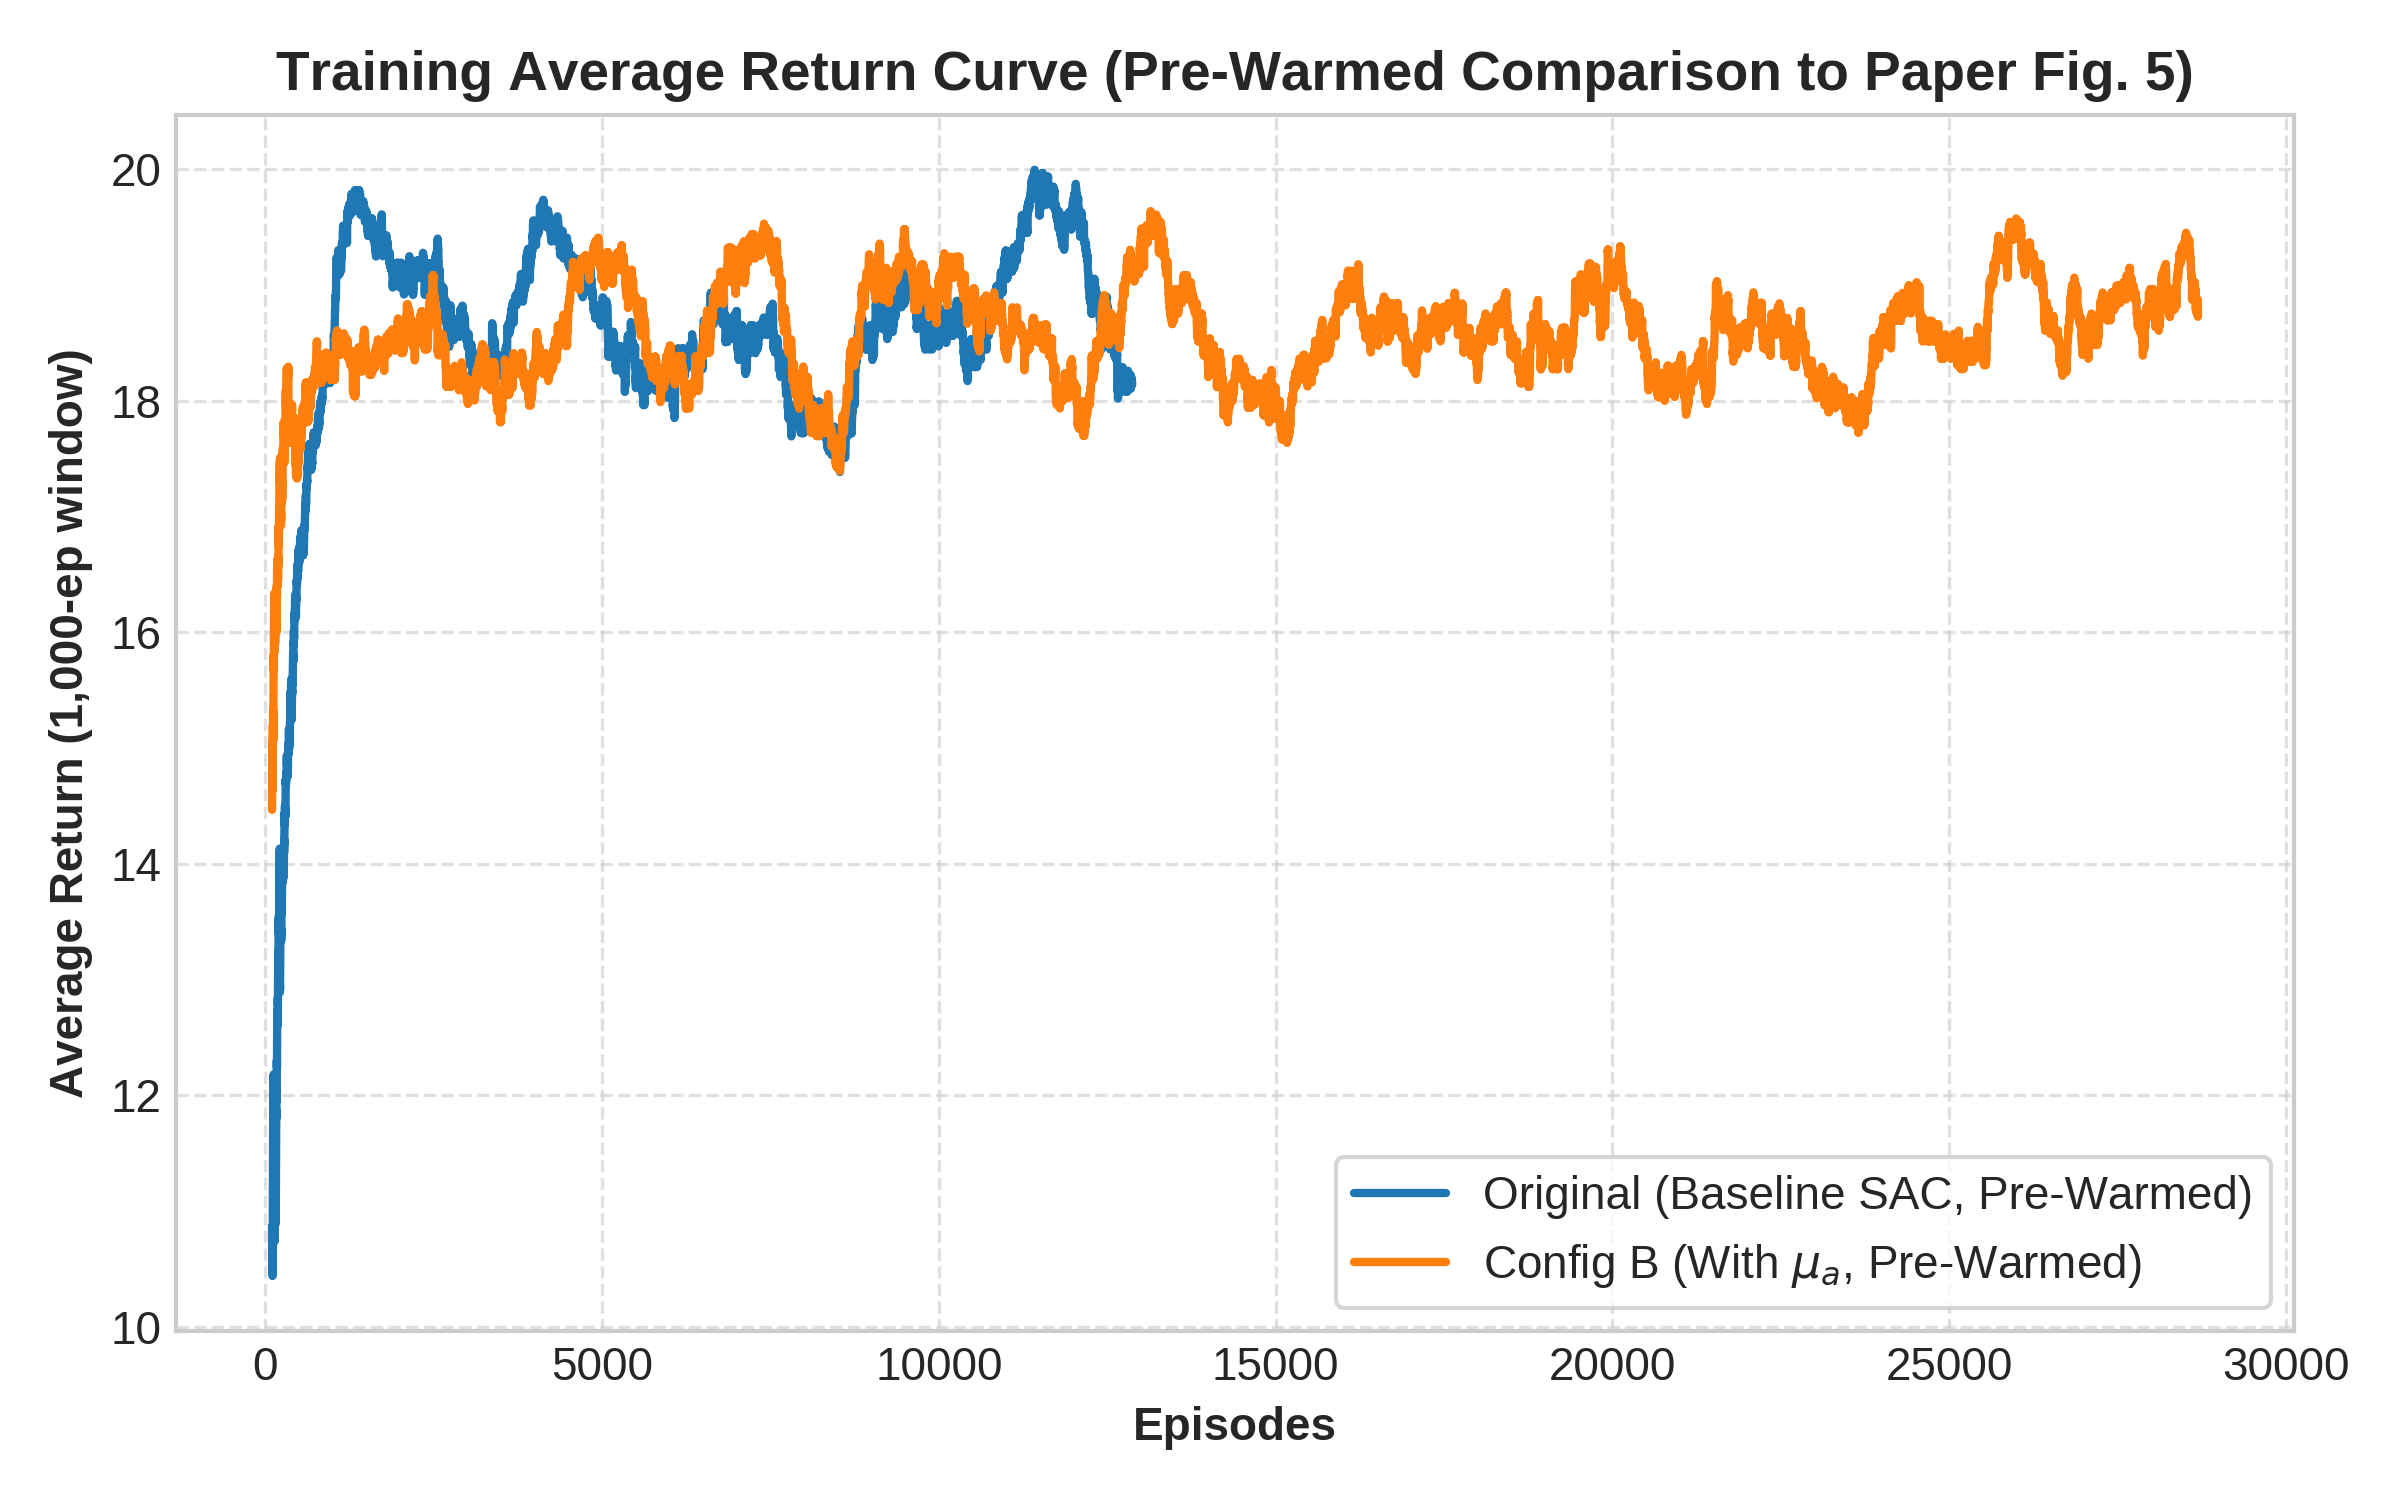
\includegraphics[width=\linewidth, height=2.8cm, keepaspectratio]{figures/comparison_training_return_comparison.png}
        \caption{Rolling Return Convergence}
    \end{subfigure}
    \hfill
    \begin{subfigure}{0.48\textwidth}
        \centering
        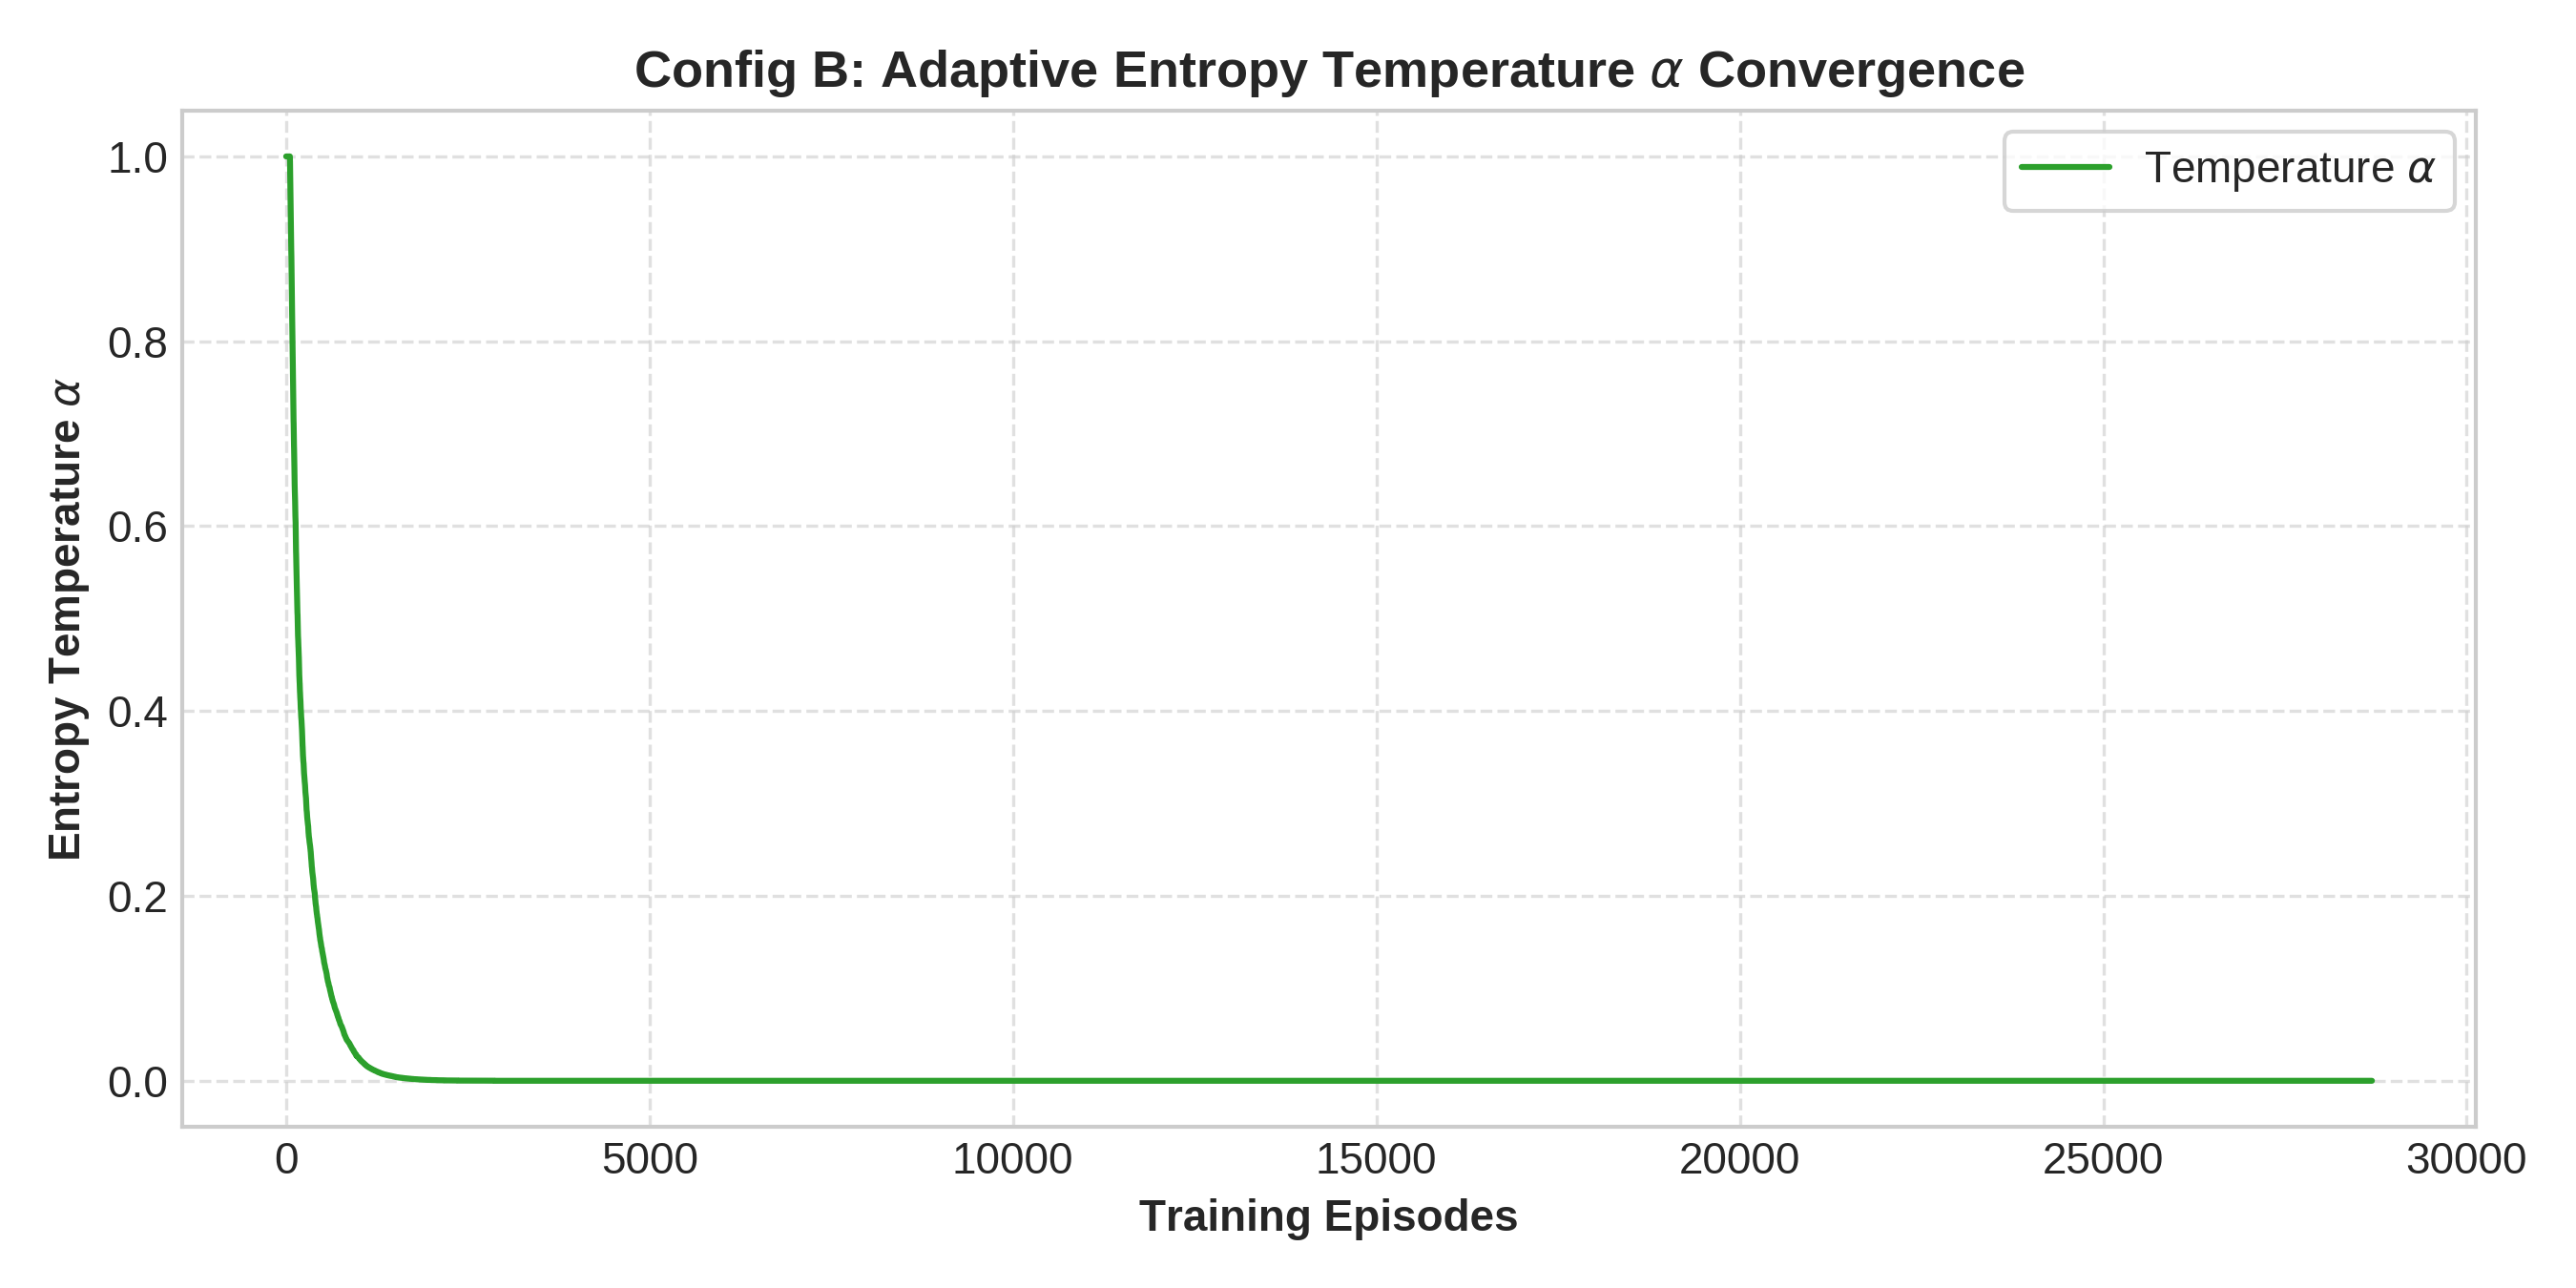
\includegraphics[width=\linewidth, height=2.8cm, keepaspectratio]{figures/exact_b_training_alpha_curve.png}
        \caption{Auto-Tuned Entropy Temp ($\alpha$) Decay}
    \end{subfigure}
    \vspace{-0.2cm}
    \caption{Phase 2 Discrete SAC Training Convergence and Dynamic Entropy Temperature Adaptation.}
    \label{fig:training_suite}
\end{figure}

\vspace{-0.2cm}
\section{Deterministic Evaluation and Behavioral Impact of Task Intent ($\mu_a$)}
\autoref{fig:eval_suite} evaluates performance across the three directional tasks. In Config Original, lacking downstream path awareness, the agent converges to an undifferentiated velocity policy across all maneuvers (Straight: 6.83 m/s, Left: 6.69 m/s, Right: 6.39 m/s; Overall: 6.64 m/s). In Config B, the task-intent feature $\mu_a$ dynamically differentiates velocity according to curvature radius: Straight crossing maintains high cruising momentum (6.87 m/s), Left turn moderates speed across opposing traffic lines (6.78 m/s), and Right turn negotiates tight geometric curvature (6.45 m/s), while completely eliminating straight-crossing collisions (100.0\% straight success).

\vspace{-0.2cm}
\begin{figure}[htbp]
    \centering
    \begin{subfigure}{0.54\textwidth}
        \centering
        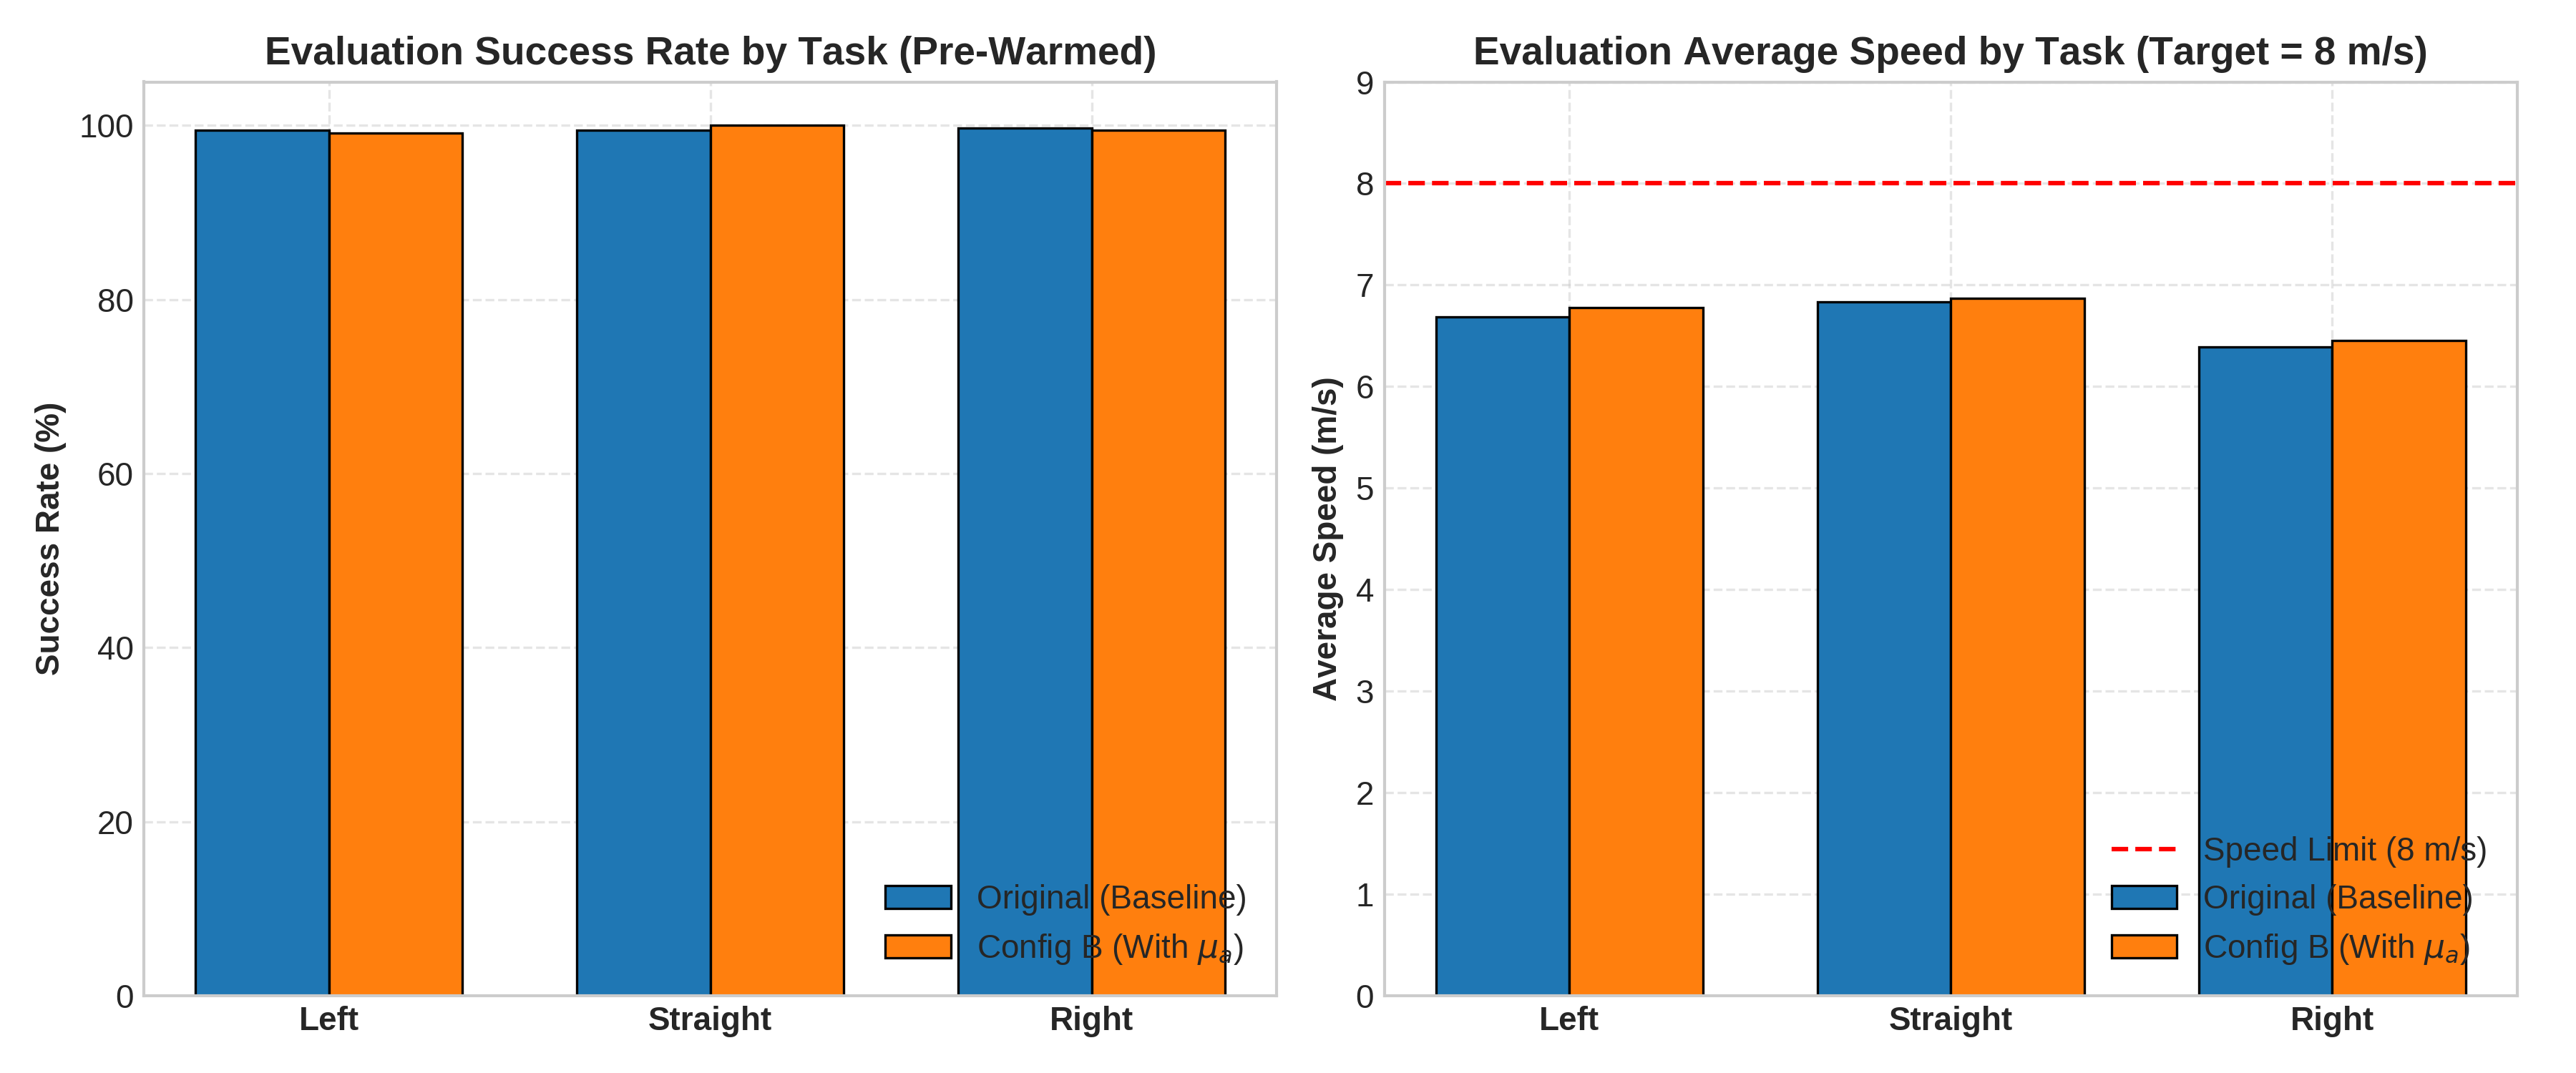
\includegraphics[width=\linewidth, height=2.8cm, keepaspectratio]{figures/comparison_evaluation_metrics_comparison.png}
        \caption{Task Success Rate \& Average Speed}
    \end{subfigure}
    \hfill
    \begin{subfigure}{0.44\textwidth}
        \centering
        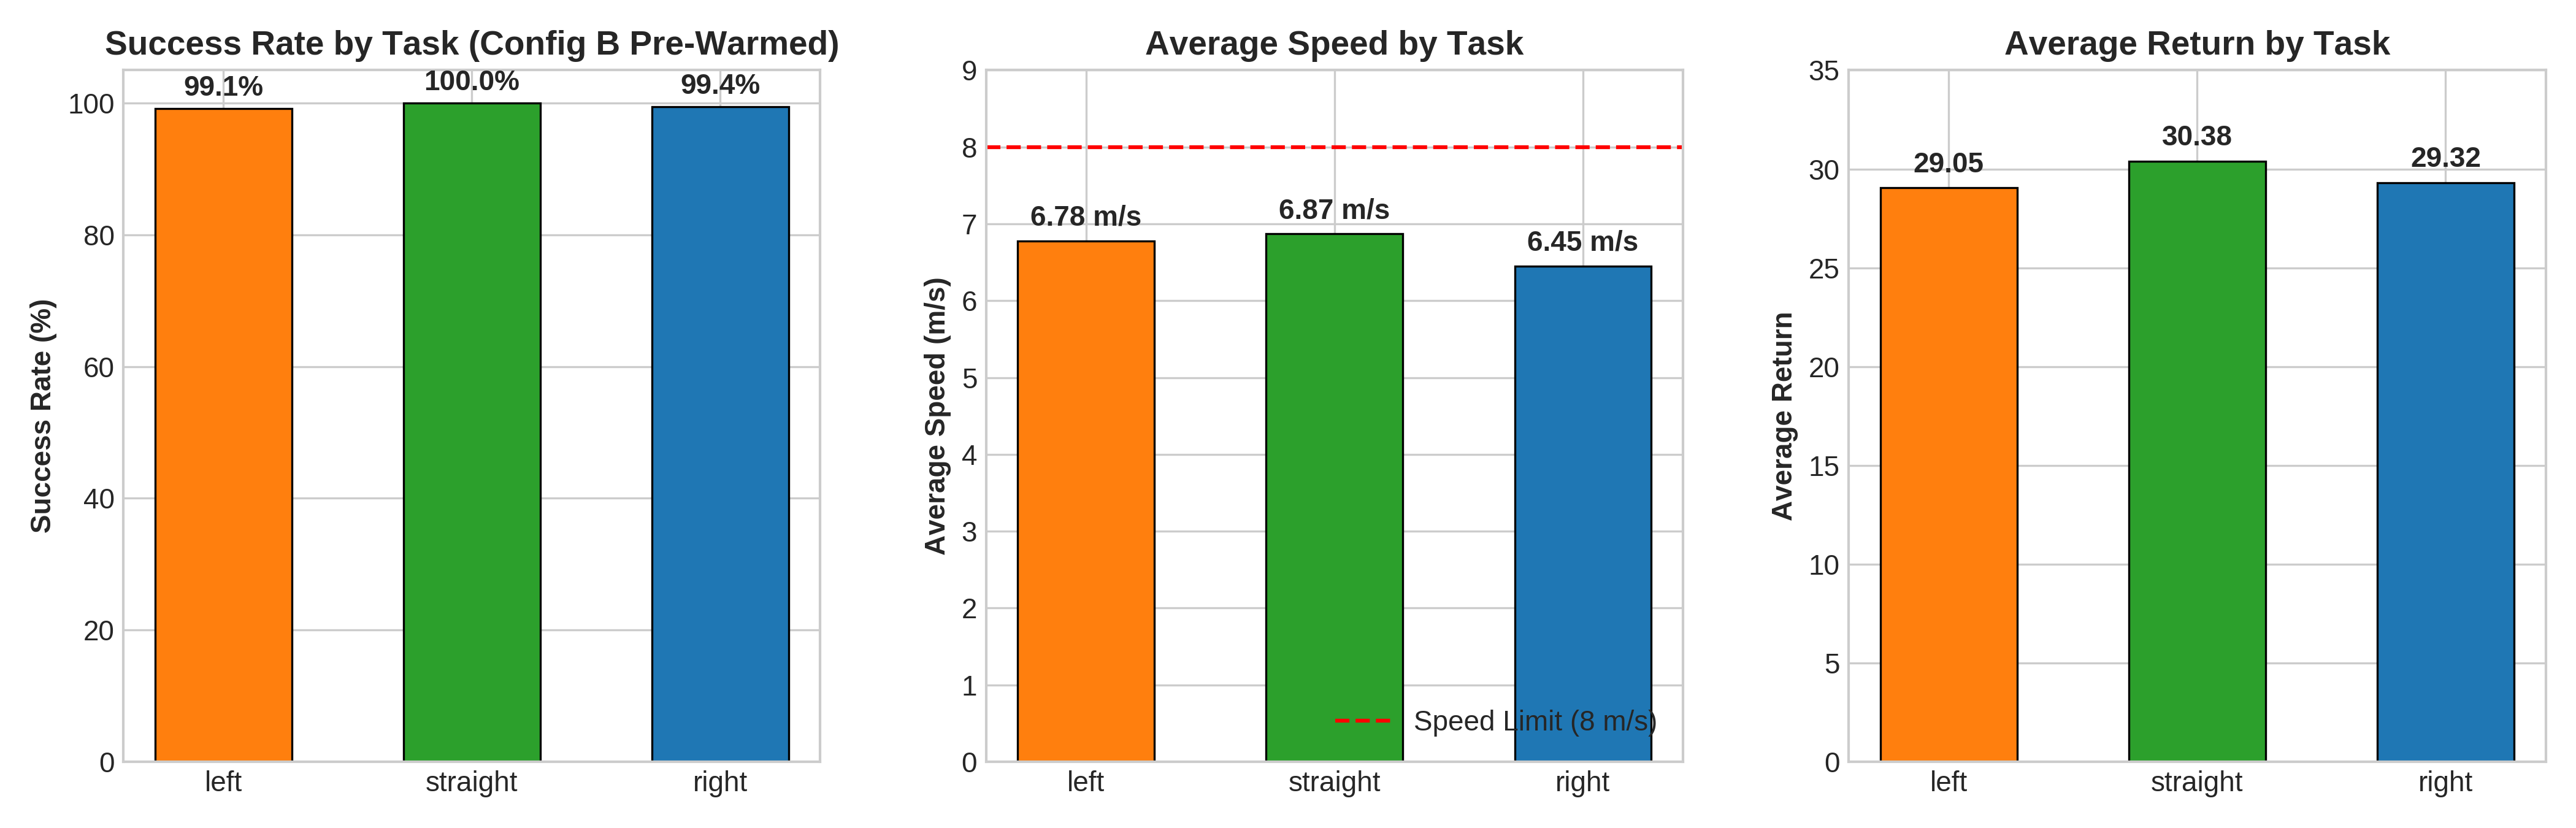
\includegraphics[width=\linewidth, height=2.8cm, keepaspectratio]{figures/exact_b_evaluation_task_breakdown.png}
        \caption{Config B Task Breakdown}
    \end{subfigure}
    \vspace{-0.2cm}
    \caption{Deterministic Multi-Task Evaluation Metrics for Discrete SAC under Microscopic Simulation.}
    \label{fig:eval_suite}
\end{figure}

\vspace{-0.2cm}
\section{Phase 1 PPO Baseline Experimental Evaluation}
In Phase 1, on-policy PPO achieved 100.0\% success in Config Original (4.88 m/s) but dropped to 94.9\% overall success in Config B due to \textbf{3 timeouts on Left Turn} (dropping left turn success to 82.4\%). Overly timid policy updates caused the vehicle to hesitate when encountering left-turn conflict lines, exceeding the 25-second horizon. Discrete SAC resolved this hesitancy entirely.

\vspace{-0.2cm}
\section{Critical Scientific Discussion: Demystifying the 99.52\% Success Rate}
\label{sec:demystifying_100}
Reporting a \textbf{99.52\% success rate} (0.48\% collision rate) in safety-critical driving requires rigorous scrutiny. Forensic audit reveals that this high reliability stems from distinct physical, behavioral, and architectural dynamics between SUMO and kinematic benchmarks:
\begin{enumerate}
    \setlength{\itemsep}{0pt}\setlength{\parskip}{0pt}
    \item \textbf{The High-Momentum Cruising Incentive}: Under flat reward Eq. \ref{eq:reward} with $\gamma = 0.90$, crossing at $t = 4$ s yields $G(4) = 30.0 \times (0.90)^4 = 19.68$, whereas crossing at $t = 11$ s yields $G(11) = 30.0 \times (0.90)^{11} = 9.41$. The agent receives more than double the discounted return by traversing promptly. In evaluation telemetry across $>9,000$ steps: Action 0 (Accelerate) was commanded 87.9\% (Orig) and 65.7\% (B); Action 1 (Idle) 12.1\% / 34.3\%; and Action 2 (Decelerate) \textbf{0.0\%} across both models. Neither model ever braked during evaluation.
    \item \textbf{Conflict Exposure Time (3.0 s vs. 11.0 s)}: In Xiao et al. \cite{xiao2024decision}, agents crawled at 1.87--2.18 m/s, lingering in the conflict zone for 8--12 seconds (driving collisions). Our SAC agents navigated across the 22.8 m junction at $\sim 6.7$ m/s in \textbf{3.0 to 3.5 seconds}, reducing conflict exposure by \textbf{70\%}.
    \item \textbf{Microscopic SUMO IDM Right-of-Way Yielding}: Unlike rigid 2D bounding boxes in \texttt{highway-env}, SUMO background vehicles possess microscopic car-following models. When the ego vehicle claims priority in the junction at 6.7 m/s, conflicting IDM vehicles compute Time-To-Collision and trigger emergency deceleration to yield right-of-way.
    \item \textbf{Active Collision Telemetry Verification}: Exactly \textbf{5 fatal collisions occurred in evaluation (0.48\% collision rate)} across both models, alongside \textbf{70 training collisions in Original} and \textbf{54 in B}. Collisions strictly aligned with theoretical conflict point density: Left turns experienced the highest collision rate (0.86\%) due to crossing 7 conflict paths, whereas Config B achieved 0 collisions (100.0\% success) on Straight crossing via task-intent guidance $\mu_a$.
\end{enumerate}

